\documentclass[tikz,border=10pt]{standalone}
\begin{document}
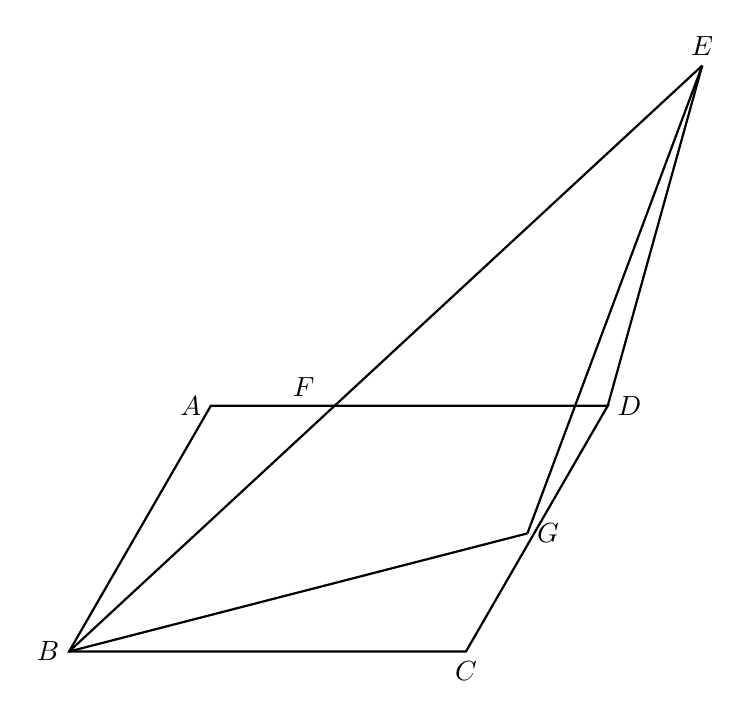
\begin{tikzpicture}[scale=1.2]
\coordinate (B) at (0,0);
\coordinate (C) at (4.2,0);
\coordinate (D) at (5.7,2.6);
\coordinate (A) at (1.5,2.6);
\coordinate (E) at (6.7,6.2);
\coordinate (F) at (2.7,2.6);
\coordinate (G) at (4.85,1.25);

\draw[thick] (A) -- (B) -- (C) -- (D) -- cycle;
\draw[thick] (B) -- (E);
\draw[thick] (E) -- (G);
\draw[thick] (B) -- (G);
\draw[thick] (E) -- (D);

\node[left] at (A) {$A$};
\node[left] at (B) {$B$};
\node[below] at (C) {$C$};
\node[right] at (D) {$D$};
\node[above] at (E) {$E$};
\node[above left] at (F) {$F$};
\node[right] at (G) {$G$};
\end{tikzpicture}
\end{document}
